\paragraph{La classe CommunicationCANdroid}

\begin{minipage}
    {\linewidth}
    \centering
    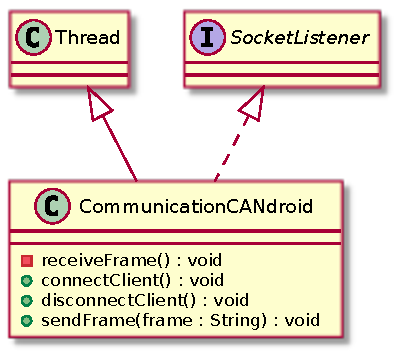
\includegraphics[width=0.5\linewidth]{../schemas/Conception_detaillee/classe_communicationCANdroid.pdf}
    \captionof{figure}{Diagramme de classe de CommunicationCANdroid}
\end{minipage}

\subparagraph{Philosophie de conception \newline} 

\medspace

La classe CommunicationCANdroid a pour rôle d'utiliser les opérations de connexion afin de faire la liaison entre le métier et le logiciel. 

\subparagraph{Description structurelle \newline}

\medspace

\textbf{Attributs :}

N.A.

\textbf{Services offerts :}

\begin{itemize}
    \item \textbf{receiveFrame() : void} --- Opération qui permet de recevoir des trames. 
    \item \textbf{connectClient() : void } --- Opération qui permet de se connecter au programme {\nomLogiciel}. 
    \item \textbf{disconnectClient() : void } --- Opération qui permet de se déconnecter au programme {\nomLogiciel}. 
    \item \textbf{sendFrame(frame : String) : void} --- Opération qui permet d'envoyer les trames au programme {\nomLogiciel}.
\end{itemize}